\documentclass{standalone}
\usepackage{tikz,amsmath}
\begin{document}
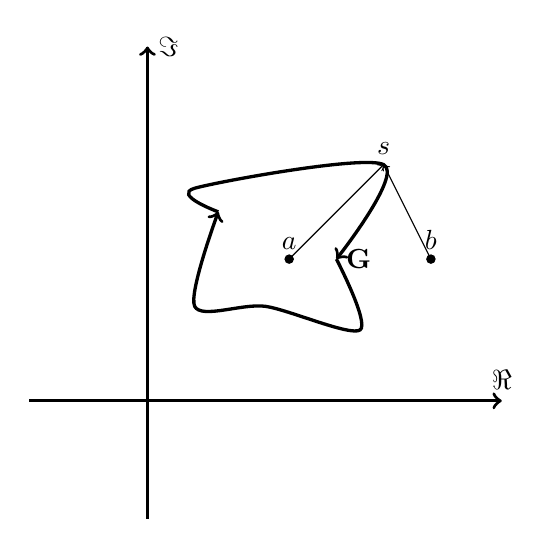
\begin{tikzpicture}[scale=3]
    \draw[->,very thick](0,-0.5)--(0,1.5)node[right]{$\Im$};
    \draw[->,very thick](-0.5,0)--(1.5,0)node[above]{$\Re$};

    \draw[->,very thick]plot[smooth]coordinates{(0.3,0.8) (0.2,0.9) (1,1) (0.8,0.6)};
    \draw[->,very thick]plot[smooth]coordinates{(0.8,0.6) (0.9,0.3) (0.5,0.4) (0.2,0.4)(0.3,0.8)};

    \node[right]at(0.8,0.6){$\mathbf{G}$};

    \node[above]at(1,1){$s$};
    \node[above]at(0.6,0.6){$a$};
    \filldraw[black](0.6,0.6)circle(0.5pt);
    \node[above]at(1.2,0.6){$b$};
    \filldraw[black](1.2,0.6)circle(0.5pt);
    
    \draw[->](0.6,0.6)--(1,1);
    \draw[->](1.2,0.6)--(1,1);
\end{tikzpicture}
\end{document}